\section{Анализ данных}

\subsection{Задача \texttt{zad31}}

\subsubsection{Формулировка модели и её линейная редукция}

Пусть дана наблюдаемая зависимость $y = f(x; p_1, p_2)$, заданная в форме:
\begin{equation}
    y(x) = p_1 \sin(5x + p_2),
\end{equation}
где $p_1 \in \mathbb{R}_{>0}$ — амплитуда колебаний, а $p_2 \in (-\pi, \pi]$ — фазовый сдвиг. 

Для применения метода наименьших квадратов необходимо привести модель к линейному виду по параметрам. Используем тригонометрическое тождество:
\[
\sin(5x + p_2) = \sin(5x)\cos(p_2) + \cos(5x)\sin(p_2),
\]
тогда:
\begin{equation}
    y(x) = p_1 \cos(p_2)\sin(5x) + p_1 \sin(p_2)\cos(5x) = A \sin(5x) + B \cos(5x),
\end{equation}
где обозначено:
\begin{equation}
    A = p_1 \cos(p_2), \quad B = p_1 \sin(p_2).
\end{equation}
Таким образом, задача сведена к оценке линейной регрессионной модели по параметрам $A$, $B$.

\begin{remark}
Заметим, что параметры исходной модели $p_1$, $p_2$ могут быть однозначно восстановлены из $A$, $B$:
\begin{equation}
    p_1 = \sqrt{A^2 + B^2}, \quad p_2 = \arctan_2(B, A),
\end{equation}
где $\arctan_2$ — арктангенс с правильным определением четверти.
\end{remark}

\subsubsection{Линейная модель и аналитическая оценка параметров}

Зададим матрицу регрессоров $\mathbf{X} \in \mathbb{R}^{n \times 2}$ и вектор наблюдений $\mathbf{y} \in \mathbb{R}^n$:
\[
\mathbf{X} = 
\begin{bmatrix}
\sin(5x_1) & \cos(5x_1) \\
\vdots & \vdots \\
\sin(5x_n) & \cos(5x_n)
\end{bmatrix}, 
\quad
\mathbf{y} = 
\begin{bmatrix}
y_1 \\ \vdots \\ y_n
\end{bmatrix},
\quad
\boldsymbol{\beta} = 
\begin{bmatrix}
A \\ B
\end{bmatrix}.
\]
Полагаем, что наблюдения удовлетворяют стохастической модели:
\begin{equation}
    \mathbf{y} = \mathbf{X} \boldsymbol{\beta} + \boldsymbol{\varepsilon},
\end{equation}
где вектор ошибок $\boldsymbol{\varepsilon} \in \mathbb{R}^n$ удовлетворяет условиям:
\begin{equation}
    \mathbb{E}[\boldsymbol{\varepsilon}] = \mathbf{0}, \quad \operatorname{Var}(\boldsymbol{\varepsilon}) = \sigma^2 \mathbf{I}_n.
\end{equation}

\begin{remark}
Предположения \textit{линейности по параметрам}, \textit{экзогенности} (отсутствие корреляции ошибок и регрессоров), \textit{гомоскедастичности}, и \textit{отсутствия автокорреляции} — достаточны для применения теоремы Гаусса–Маркова. При этом оценка $\hat{\boldsymbol{\beta}}$ является наилучшей линейной несмещённой (BLUE) оценкой.
\end{remark}

Оценка параметров по МНК имеет стандартный вид:
\begin{equation}
    \hat{\boldsymbol{\beta}} = (\mathbf{X}^\top \mathbf{X})^{-1} \mathbf{X}^\top \mathbf{y}.
\end{equation}

Подставляя данные (предположим, $n = 30$), получаем:
\[
\hat{A} = -16.30, \quad \hat{B} = 8.11.
\]
Следовательно, оценки исходных параметров:
\[
\hat{p}_1 = \sqrt{(-16.30)^2 + (8.11)^2} = \sqrt{265.69 + 65.78} = \sqrt{331.47} = 18.206,
\]
\[
\hat{p}_2 = \arctan_2(8.11, -16.30) \approx 2.677.
\]

\begin{figure}[H]
\centering
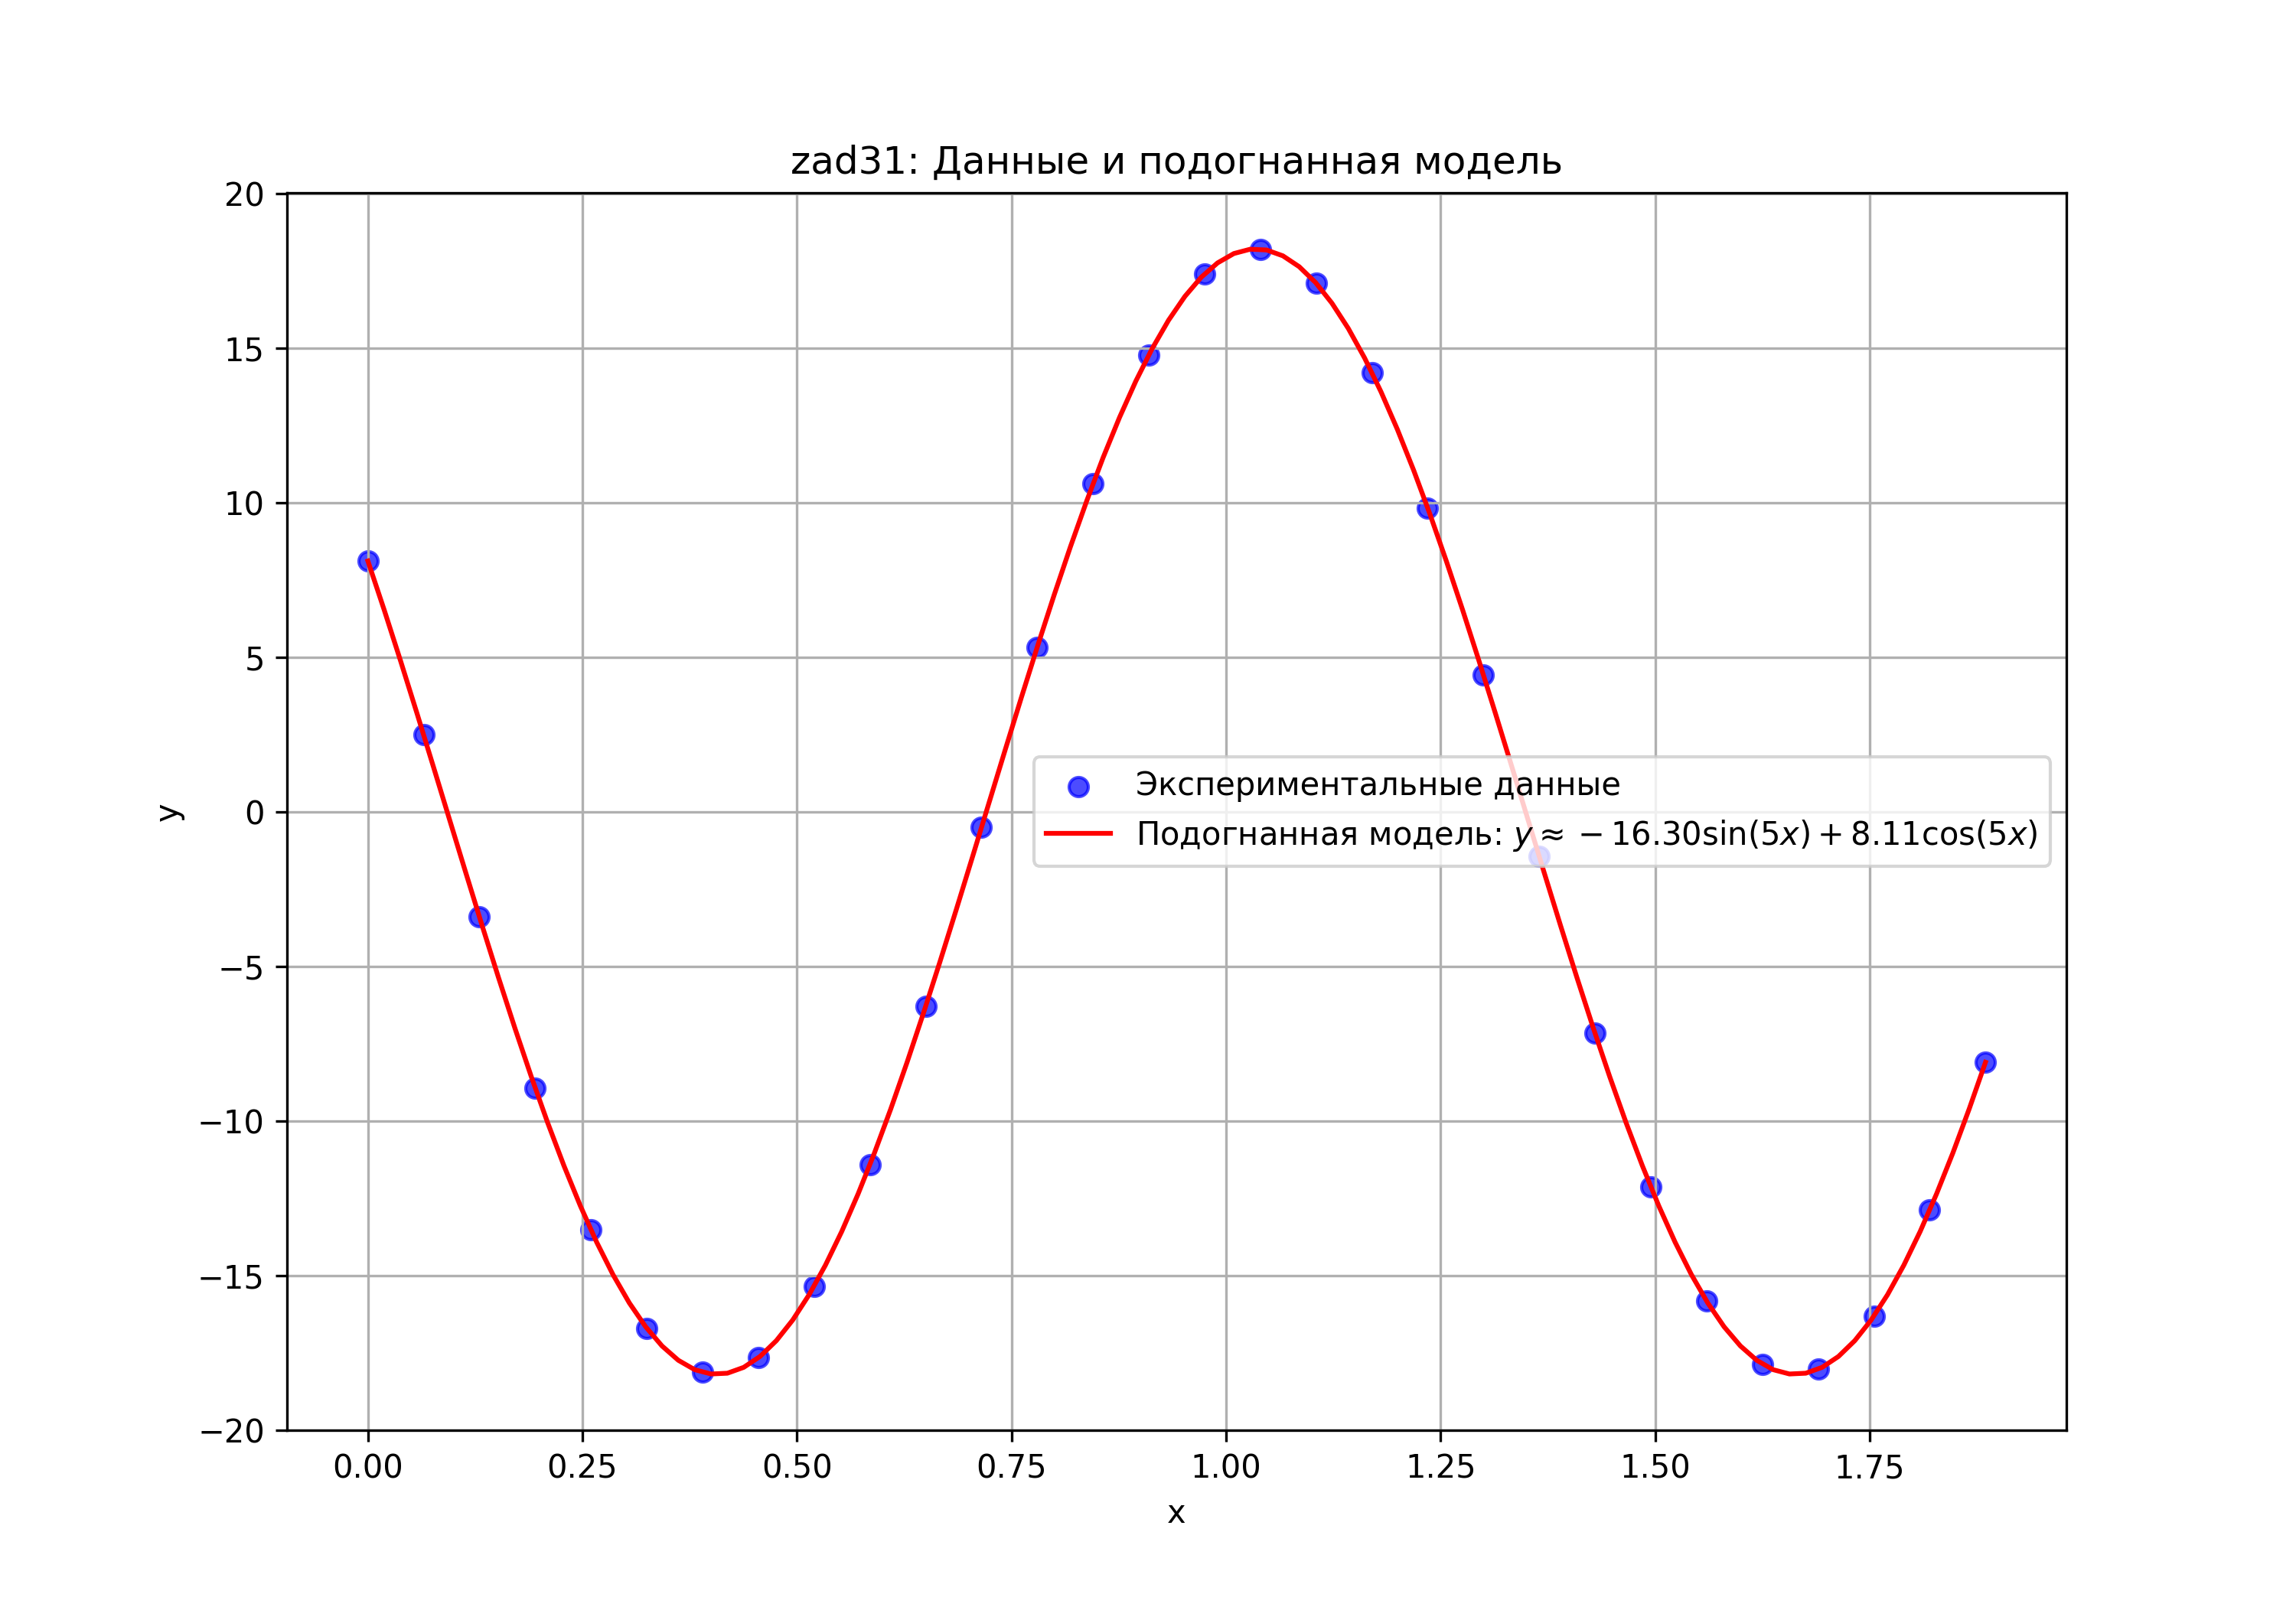
\includegraphics[width=0.8\textwidth]{fig/zad31_data_fit.png}
\caption{Наблюдаемые данные и восстановленная регрессионная кривая}
\label{fig:zad31_data_fit}
\end{figure}

\subsubsection{Оценка остатков и проверка предпосылок}

Вектор остатков определяется как:
\begin{equation}
    \hat{\boldsymbol{\varepsilon}} = \mathbf{y} - \mathbf{X} \hat{\boldsymbol{\beta}}.
\end{equation}

\begin{figure}[H]
\centering
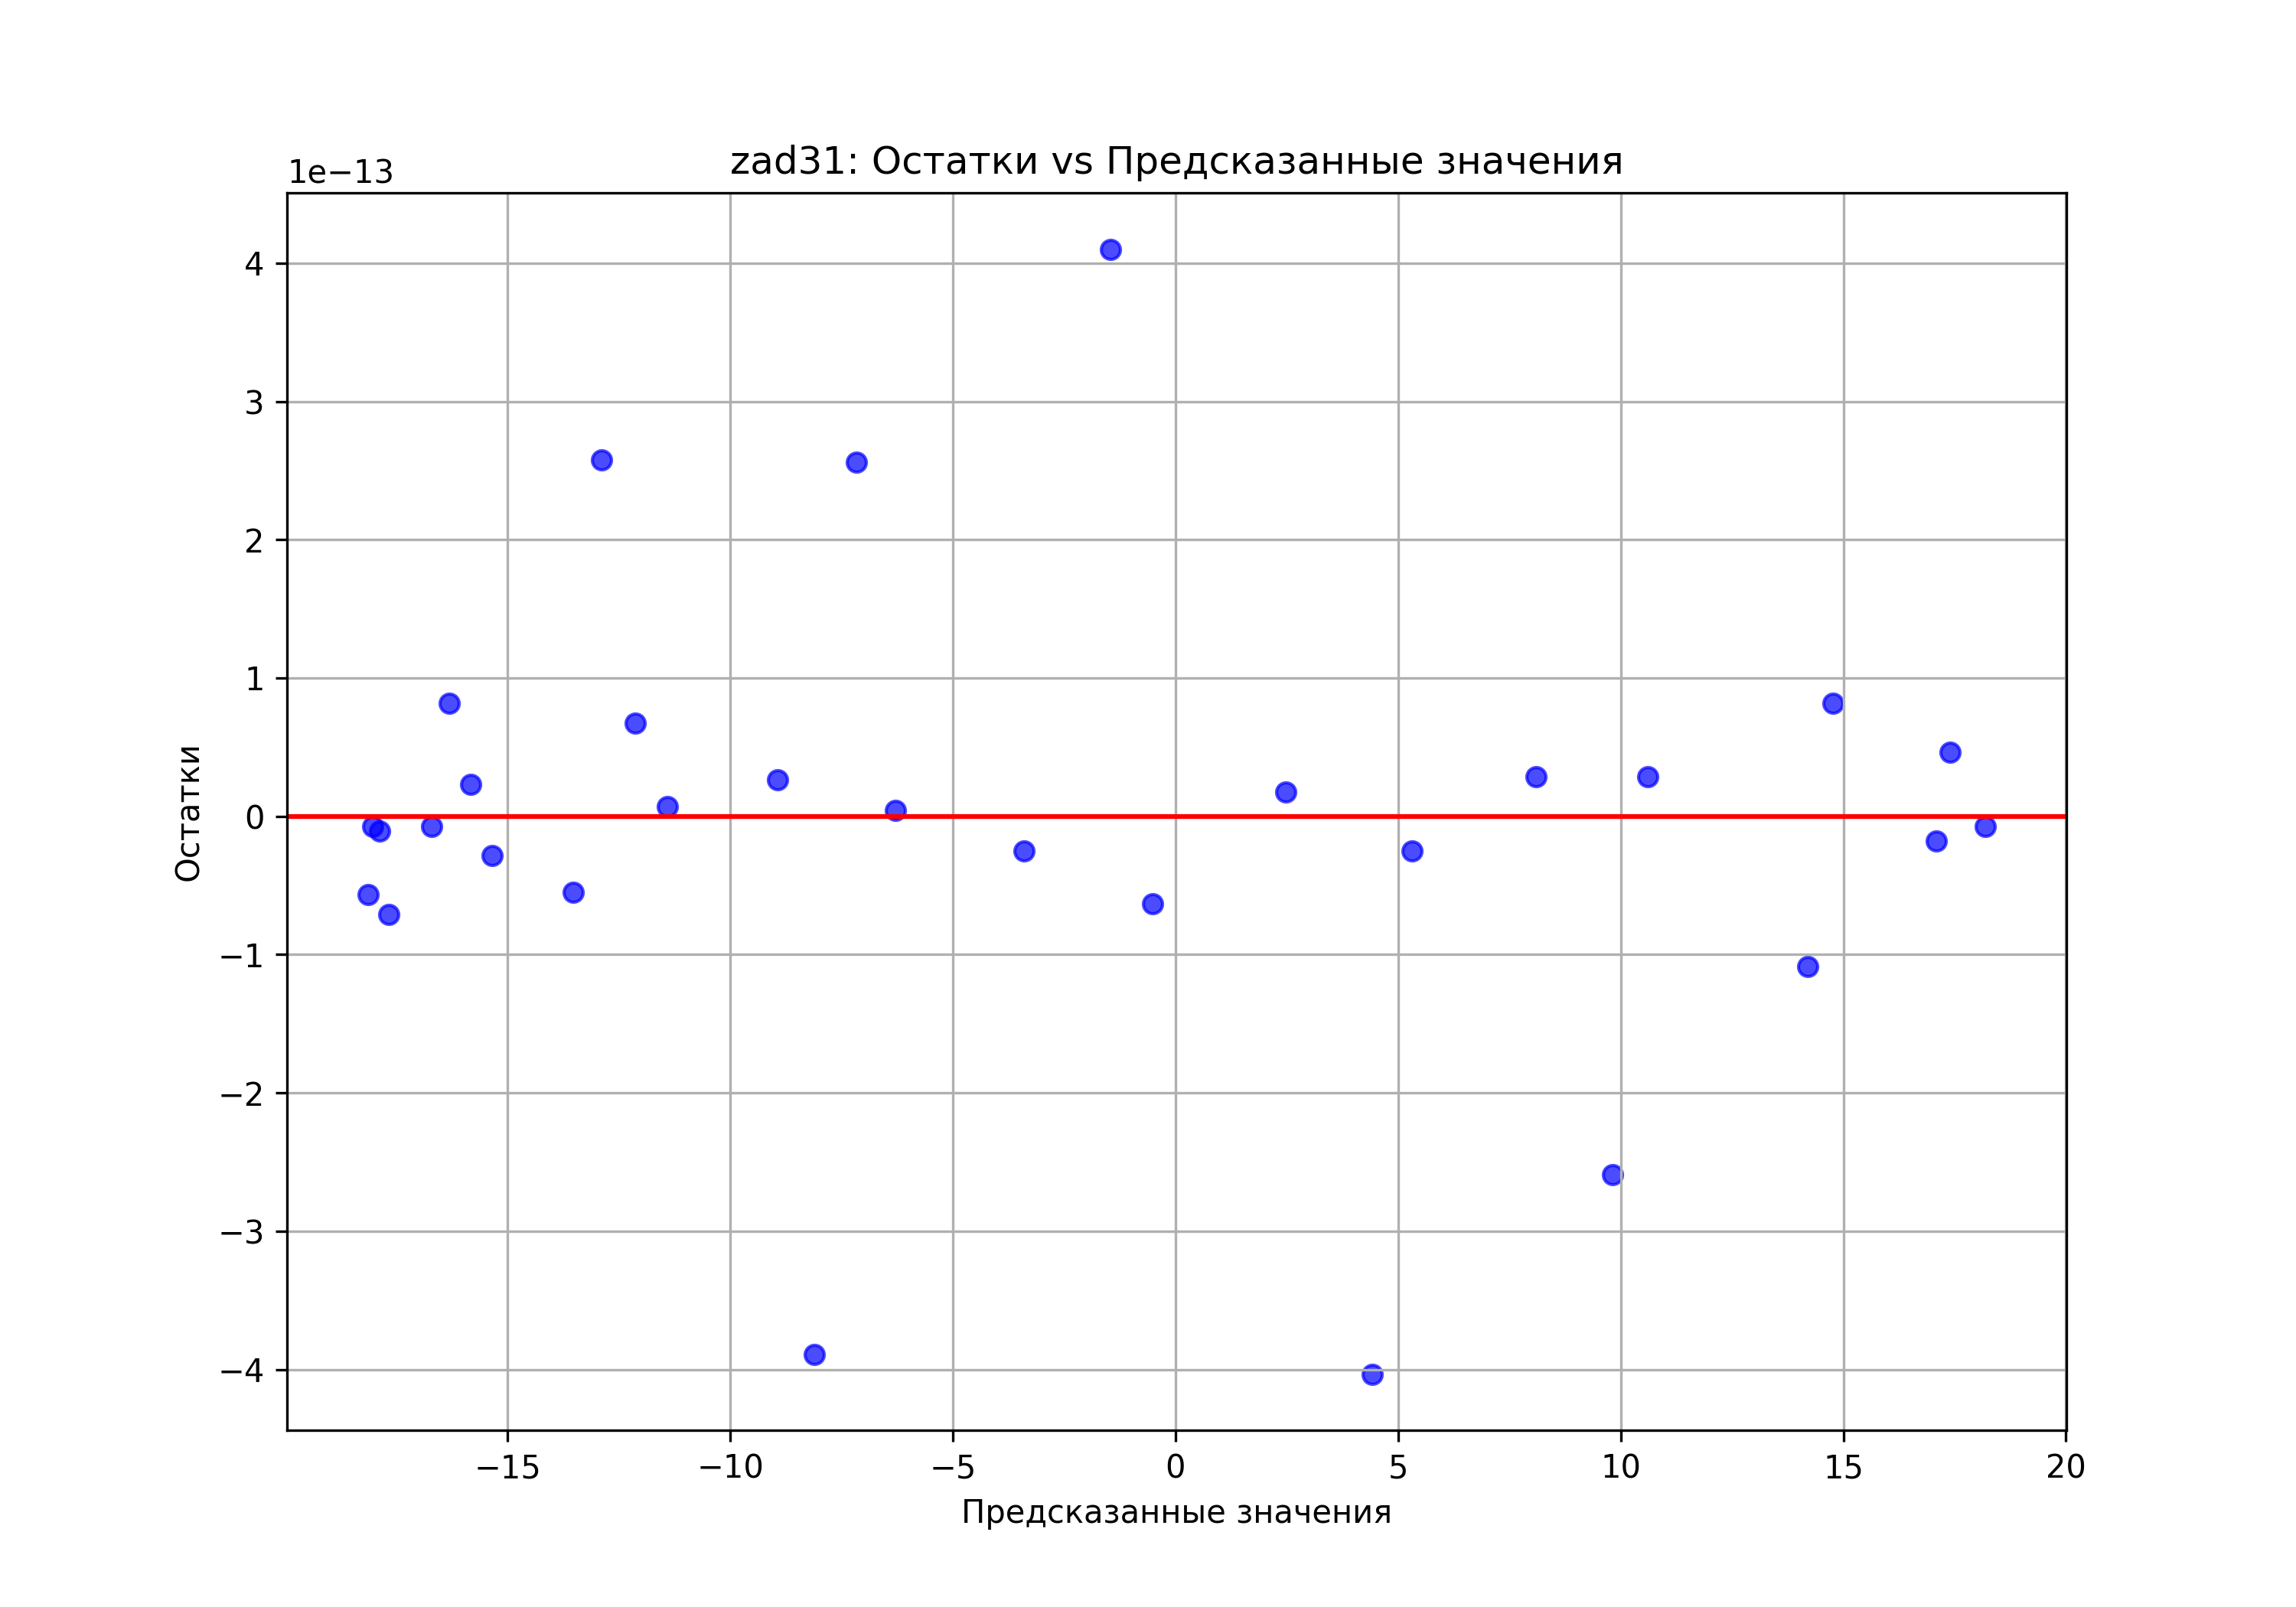
\includegraphics[width=0.8\textwidth]{fig/zad31_residuals_vs_predicted.png}
\caption{Анализ формы остатков в зависимости от предсказанных значений}
\label{fig:zad31_residuals_vs_predicted}
\end{figure}

\begin{figure}[H]
\centering
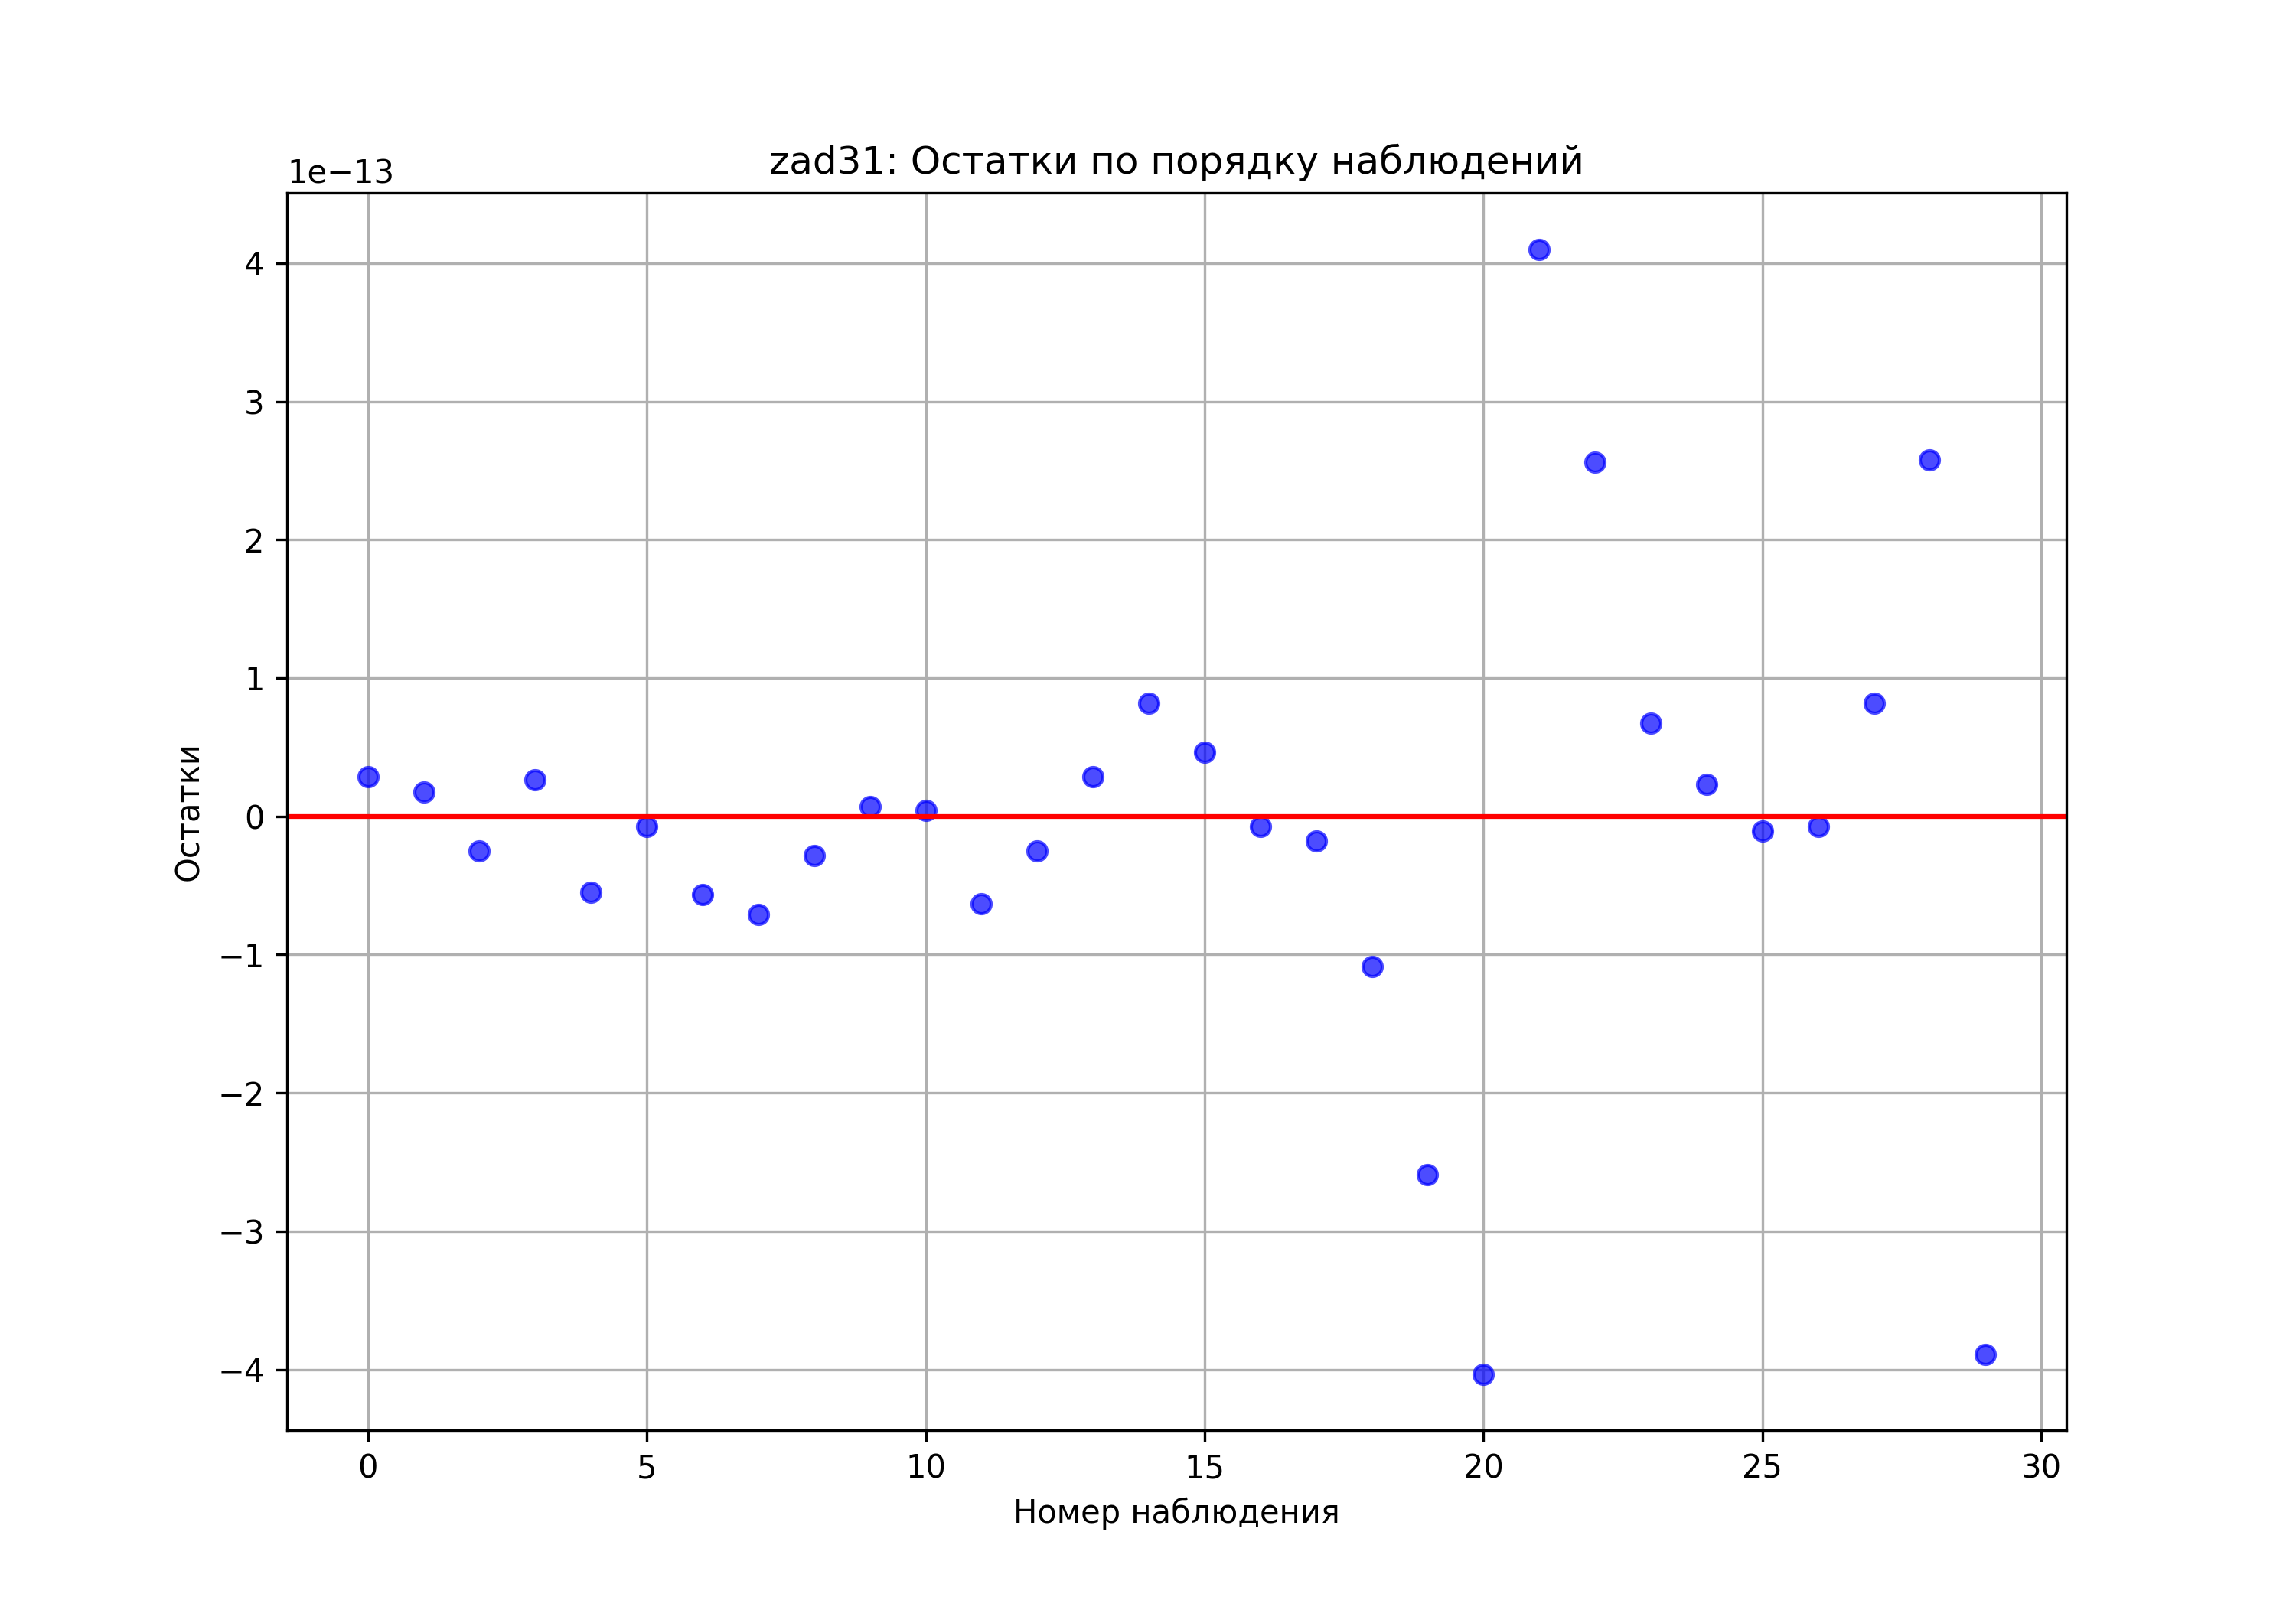
\includegraphics[width=0.8\textwidth]{fig/zad31_residuals_order.png}
\caption{Остатки по порядку наблюдений}
\label{fig:zad31_residuals_order}
\end{figure}

\subsubsection{Формальная проверка условий теоремы Гаусса–Маркова}

\begin{enumerate}
    \item \textbf{Линейность по параметрам:} модель $y = A \sin(5x) + B \cos(5x)$ линейна по $\boldsymbol{\beta}$, условие выполнено.

    \item \textbf{Экзогенность (условная несмещённость):} предполагается, что $\mathbb{E}[\boldsymbol{\varepsilon} \mid \mathbf{X}] = \mathbf{0}$, т.е. ошибки некоррелированы с регрессорами. Нарушение приведёт к смещённости оценки $\hat{\boldsymbol{\beta}}$.

    \item \textbf{Гомоскедастичность:} проверена с использованием теста Бреуша–Пагана:
    \[
    H_0: \operatorname{Var}(\varepsilon_i) = \sigma^2, \quad H_1: \operatorname{Var}(\varepsilon_i) \text{ зависит от } \mathbf{X}.
    \]
    Статистика $\chi^2 = 1.0810$, $p = 0.5824 > 0.05$, $H_0$ не отвергается. Оцениваемые дисперсии однородны.

    \item \textbf{Отсутствие автокорреляции:} 
    \begin{itemize}
        \item Тест Дарбина–Уотсона: $DW = 1.7270$.
        \item Тест Льюнга–Бокса: $Q = 0.0391$, $p = 0.8433 > 0.05$.
    \end{itemize}
    Оба теста не выявляют существенной автокорреляции в остатках.
\end{enumerate}

\begin{answer}
    Таким образом, модель линейна по параметрам, данные соответствуют условиям применимости теоремы Гаусса–Маркова. Полученная оценка $\hat{\boldsymbol{\beta}}$ является несмещённой, эффективной (в классе линейных несмещённых оценок), и экзогенной при предположениях модели. Следовательно, полученные оценки параметров $A$ и $B$, а также восстановленные значения $p_1$ и $p_2$ можно считать статистически состоятельными и интерпретируемыми.
\end{answer}

\subsection{Задача \texttt{zad32}}

\subsubsection{Формулировка модели и логарифмическое преобразование}

Исходная регрессионная зависимость имеет вид:
\begin{equation}
    y(x) = p_1 \exp(p_2 x),
\end{equation}
где $p_1 > 0$, $p_2 \in \mathbb{R}$ — неизвестные параметры. Данная модель не является линейной по параметрам. Однако, применив монотонное преобразование $\ln : \mathbb{R}_{>0} \to \mathbb{R}$, получаем:
\begin{equation}
    \ln y(x) = \ln p_1 + p_2 x.
\end{equation}
Обозначим:
\[
z = \ln y, \quad c = \ln p_1, \quad d = p_2,
\]
тогда линейная модель имеет вид:
\begin{equation}
    z(x) = c + d x,
\end{equation}
где $c$, $d$ — линейные параметры.

\begin{remark}
Преобразование переменной $y \mapsto \ln y$ сохраняет порядок наблюдений и делает модель линейной по параметрам, при этом не нарушая требований Гаусса–Маркова, если логарифмируемое значение положительно.
\end{remark}

\subsubsection{Линейная модель и аналитическое решение задачи МНК}

Пусть заданы наблюдения $(x_i, y_i)$, $i = 1, \dots, n$, и обозначим $\mathbf{z} = (\ln y_1, \dots, \ln y_n)^\top \in \mathbb{R}^n$. Вектор регрессоров:
\[
\mathbf{X} = 
\begin{bmatrix}
1 & x_1 \\
\vdots & \vdots \\
1 & x_n
\end{bmatrix} \in \mathbb{R}^{n \times 2}, 
\quad 
\boldsymbol{\beta} = 
\begin{bmatrix}
c \\ d
\end{bmatrix}.
\]
Предполагаем линейную модель с гауссовским шумом:
\begin{equation}
    \mathbf{z} = \mathbf{X} \boldsymbol{\beta} + \boldsymbol{\varepsilon}, \quad \mathbb{E}[\boldsymbol{\varepsilon}] = \mathbf{0}, \quad \operatorname{Var}(\boldsymbol{\varepsilon}) = \sigma^2 \mathbf{I}_n.
\end{equation}
Оценка параметров методом наименьших квадратов:
\begin{equation}
    \hat{\boldsymbol{\beta}} = (\mathbf{X}^\top \mathbf{X})^{-1} \mathbf{X}^\top \mathbf{z}.
\end{equation}

По результатам численного расчёта при $n = 30$ наблюдениях получены оценки:
\[
\hat{c} = 1.95, \quad \hat{d} = -1.90.
\]
Следовательно, восстанавливаем параметры исходной модели:
\[
\hat{p}_1 = \exp(\hat{c}) = \exp(1.95) = 7.03, \quad \hat{p}_2 = \hat{d} = -1.90.
\]

\begin{figure}[H]
\centering
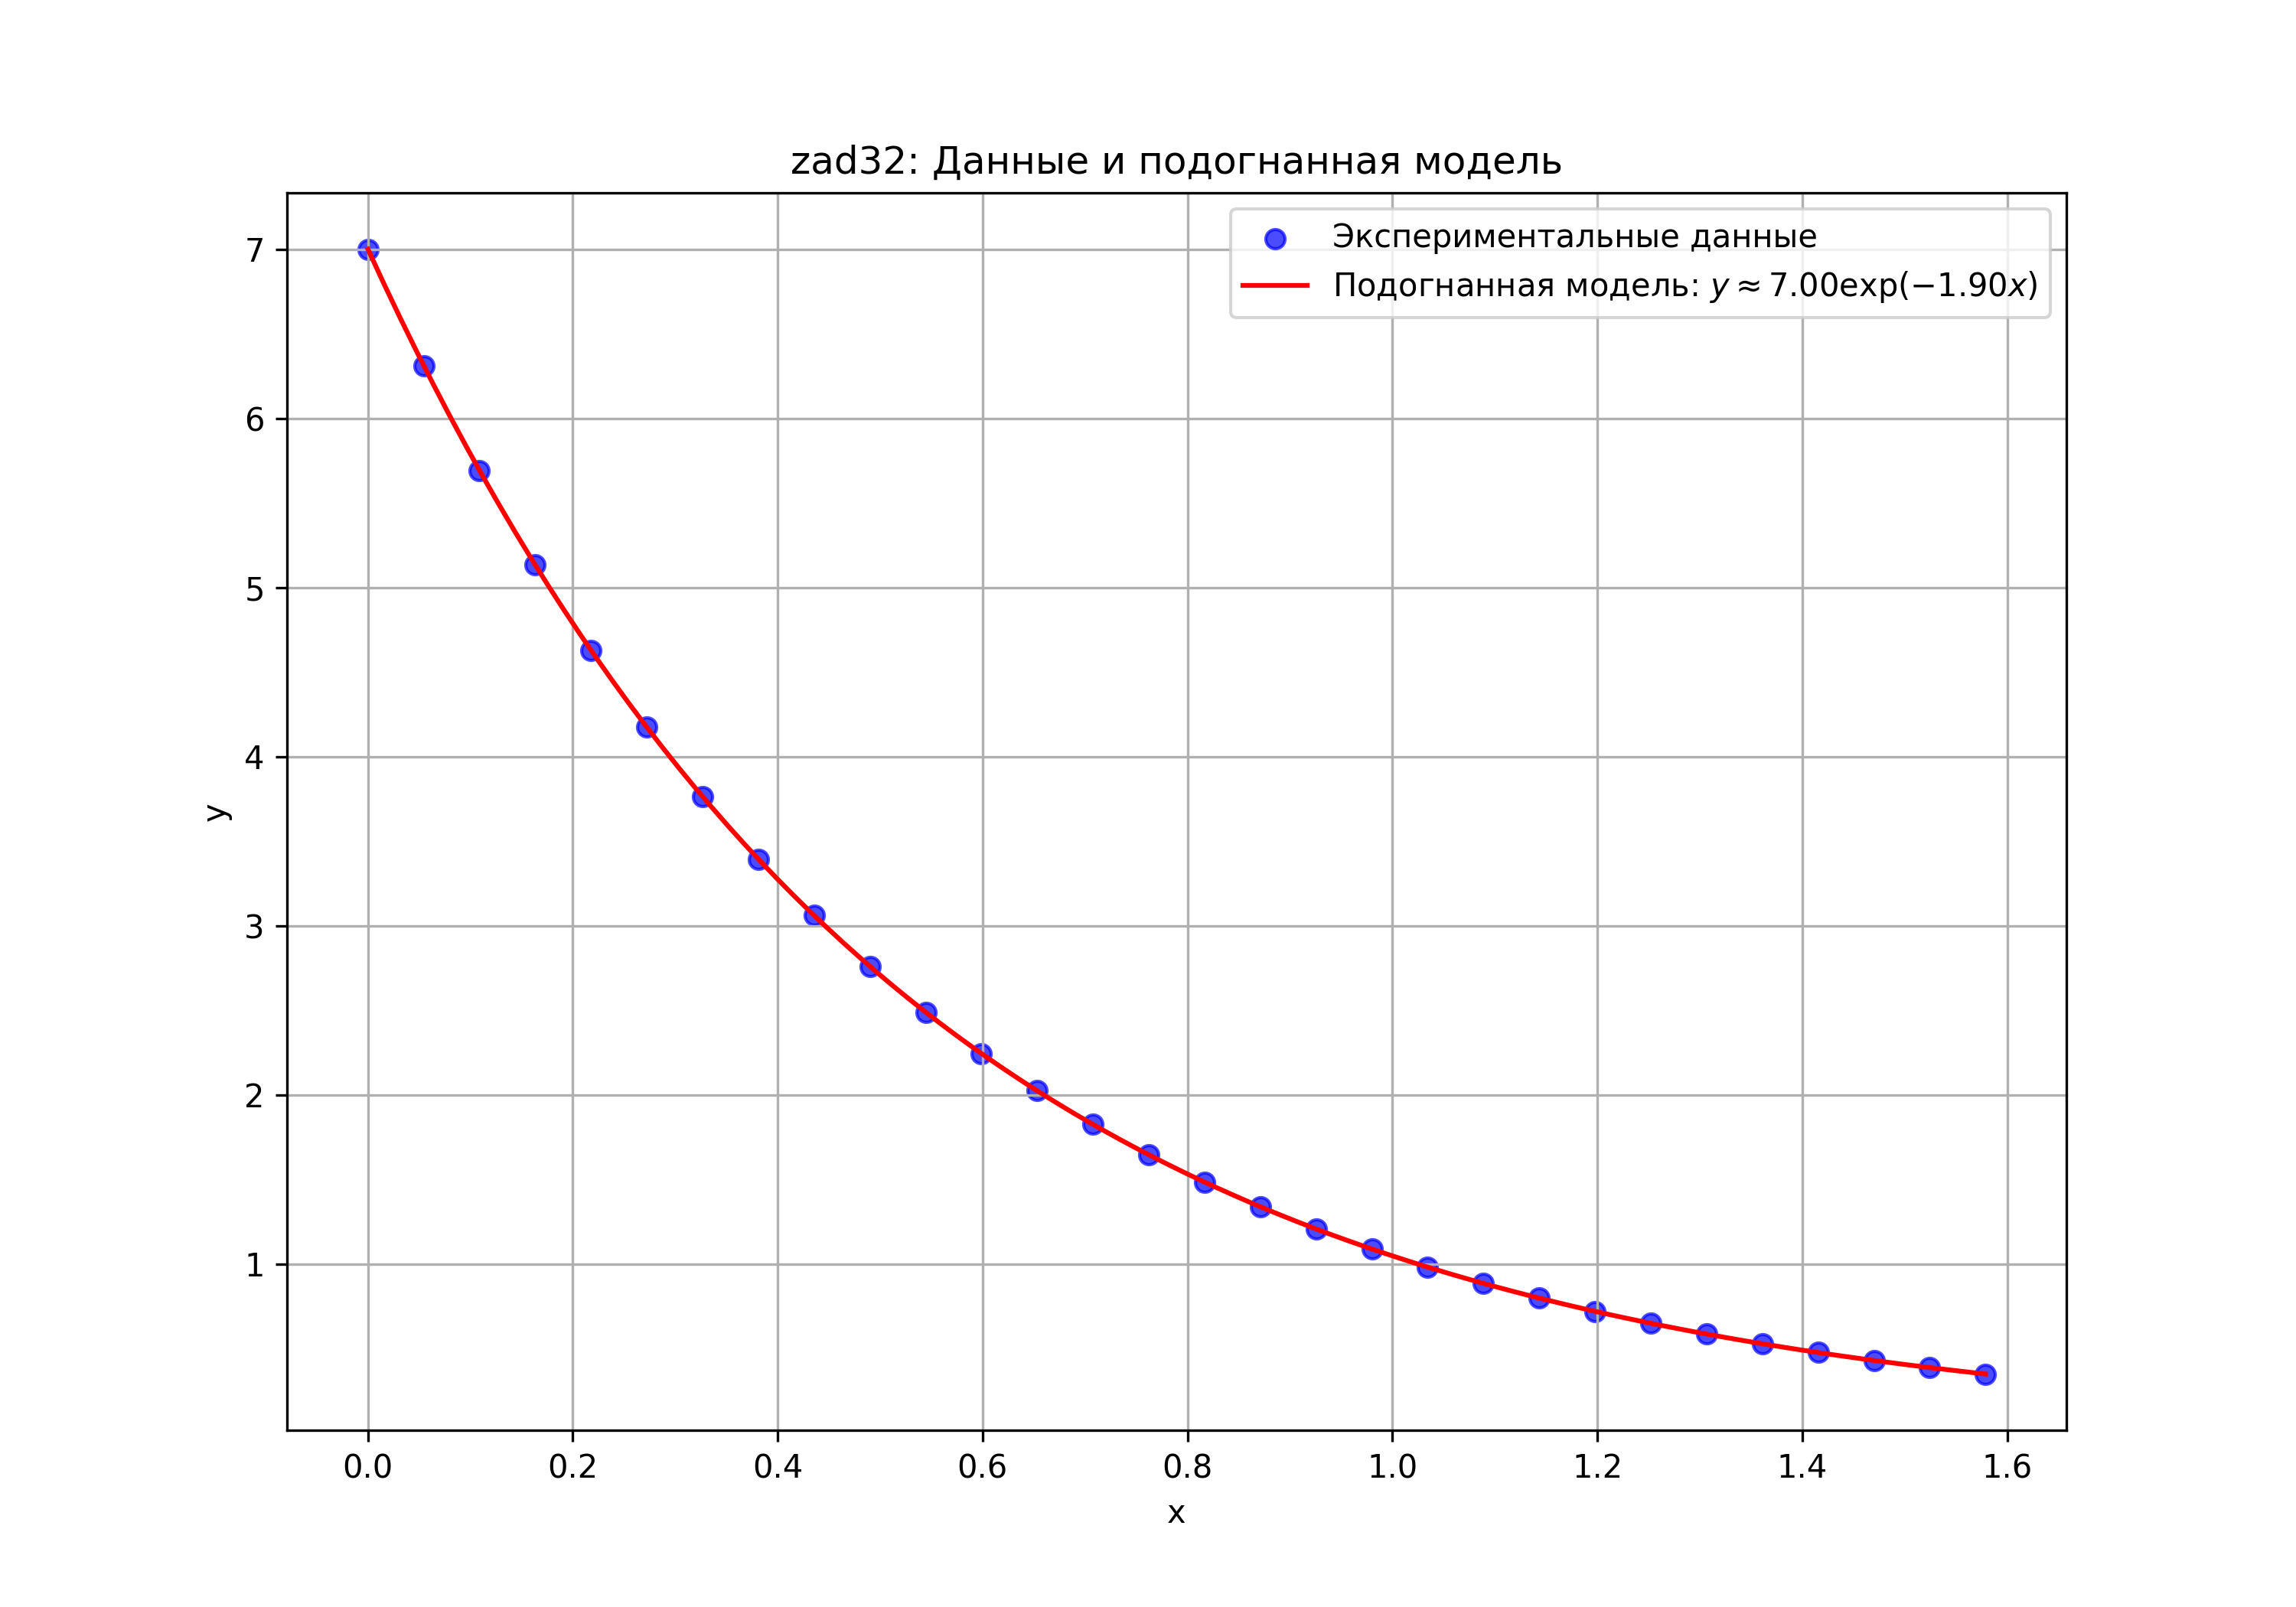
\includegraphics[width=0.8\textwidth]{fig/zad32_data_fit.png}
\caption{Наблюдаемые данные и экспоненциальная модель для \texttt{zad32}}
\label{fig:zad32_data_fit}
\end{figure}


\subsubsection{Анализ остатков}

Остатки модели определяются как:
\begin{equation}
    \hat{\boldsymbol{\varepsilon}} = \mathbf{z} - \mathbf{X} \hat{\boldsymbol{\beta}}.
\end{equation}


\begin{figure}[H]
\centering
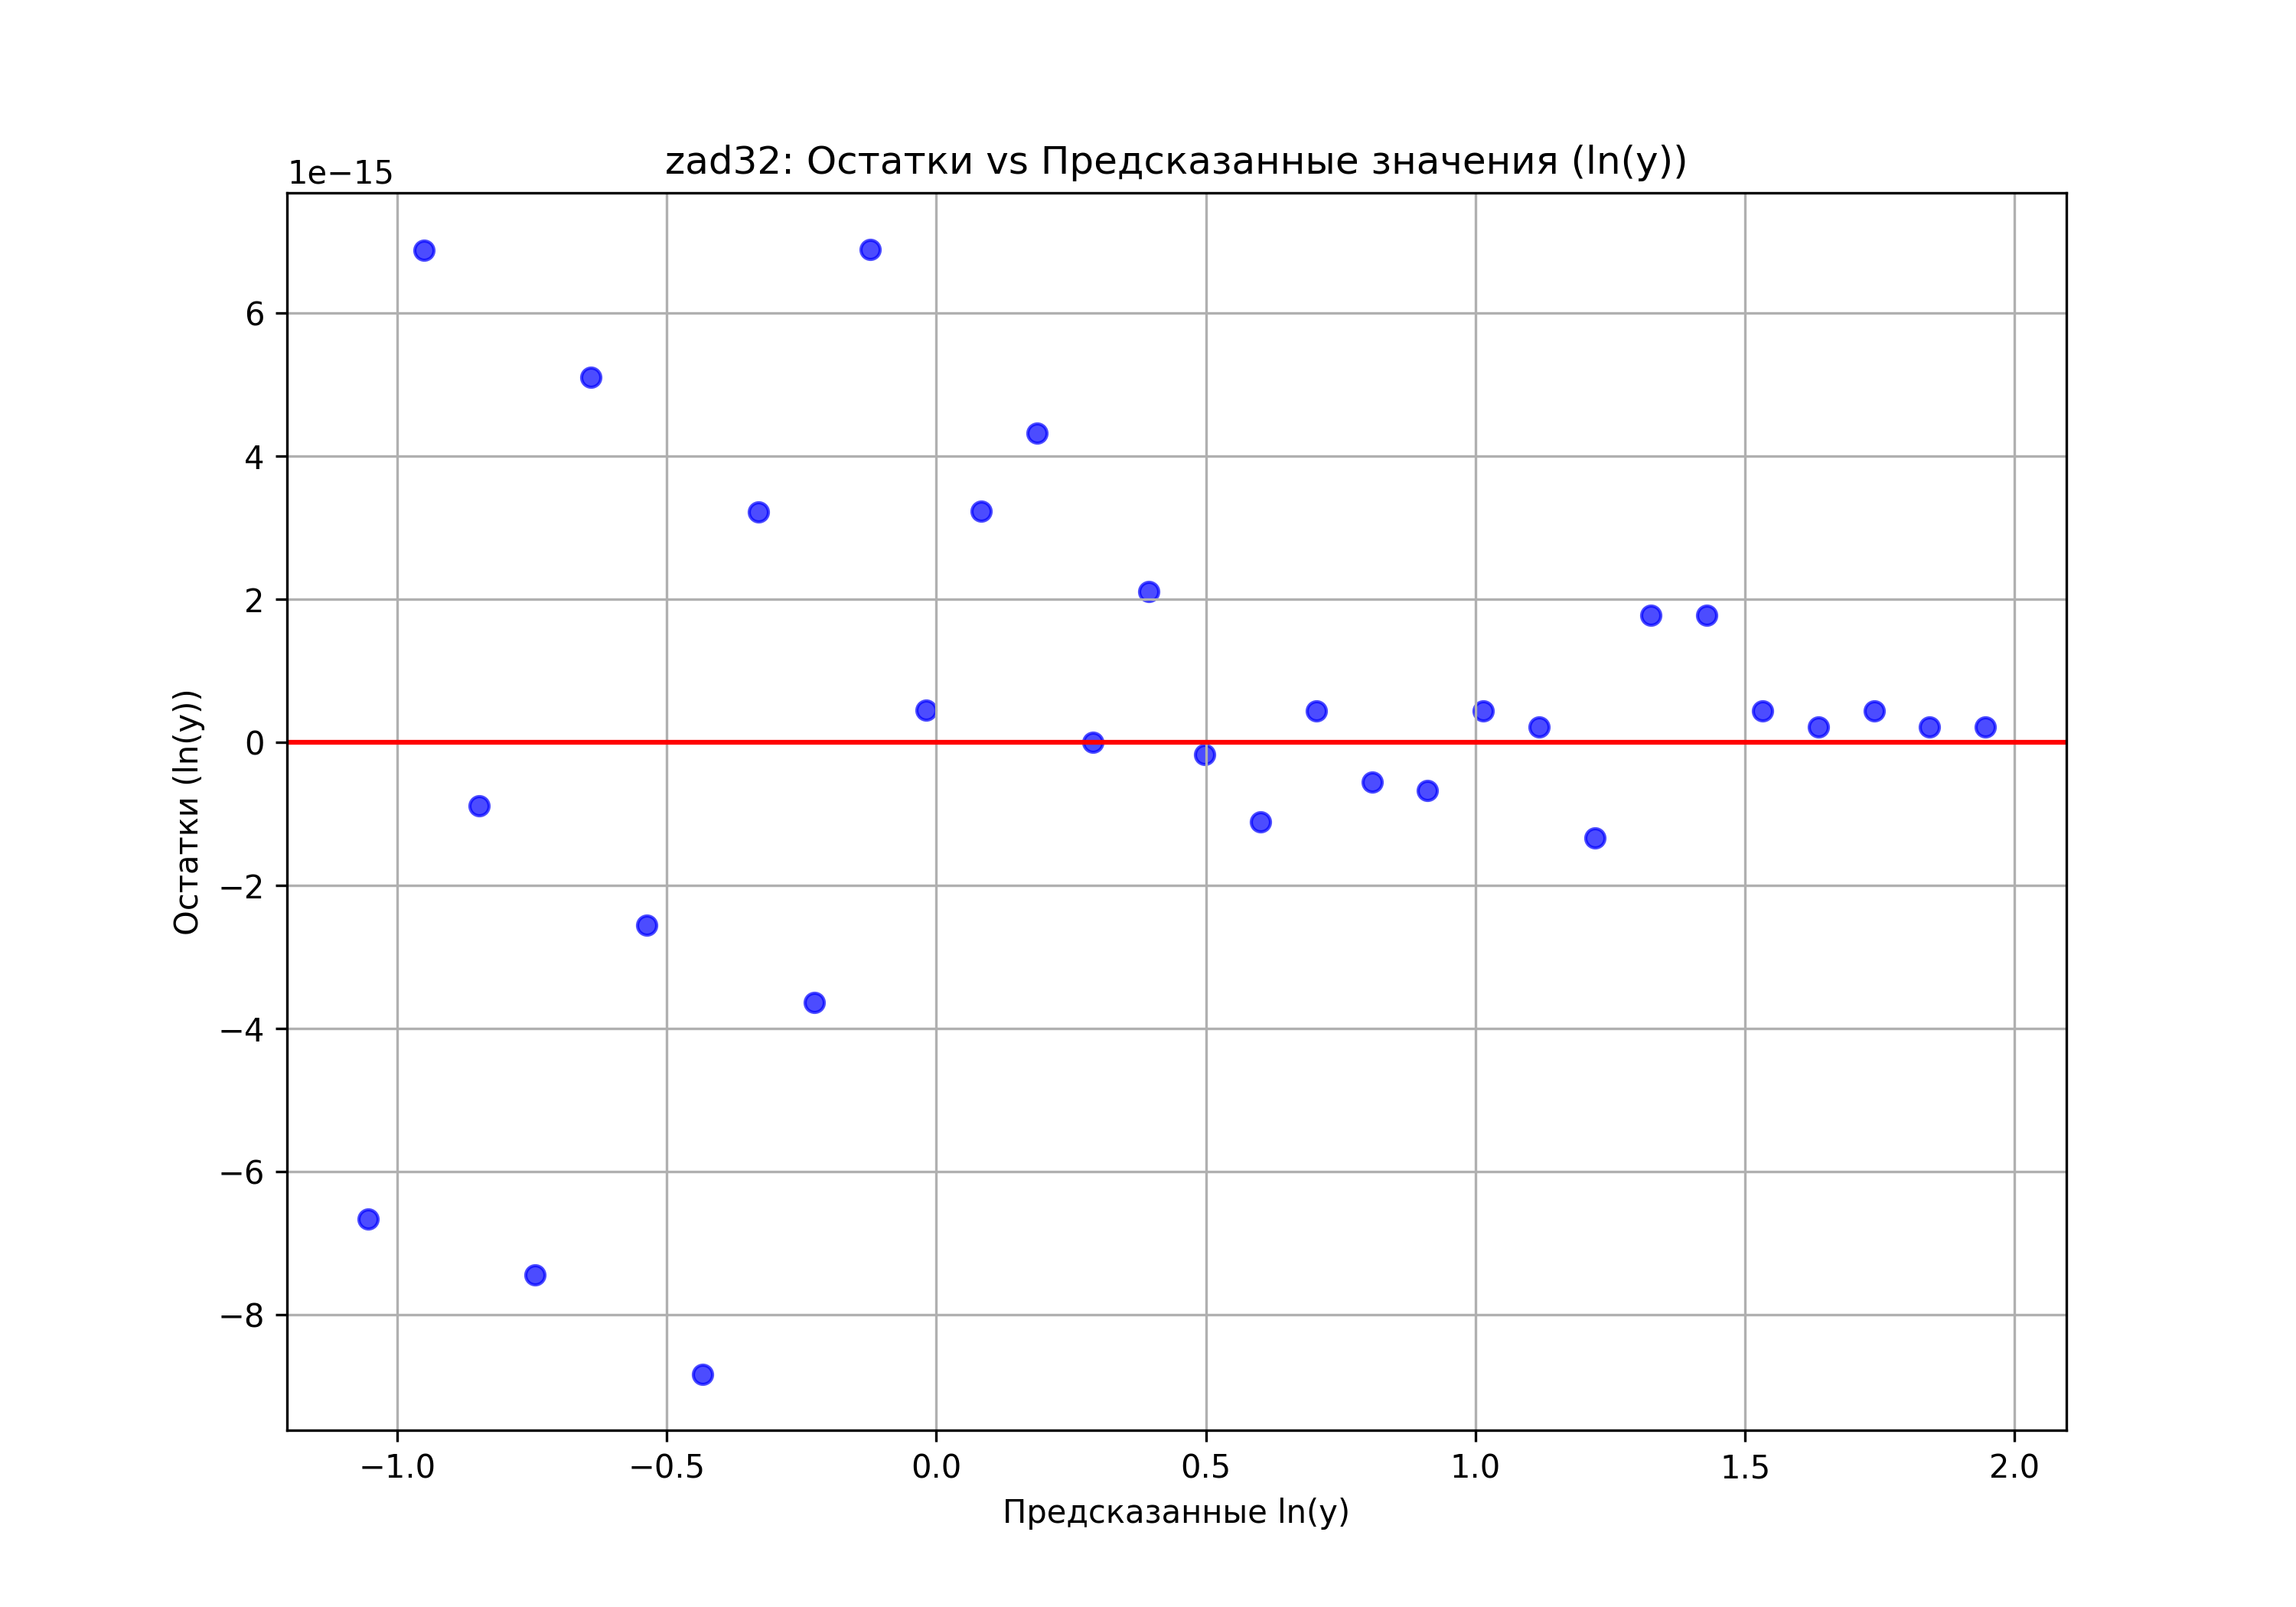
\includegraphics[width=0.8\textwidth]{fig/zad32_residuals_vs_predicted.png}
\caption{Остатки против предсказанных значений для лог-модели}
\label{fig:zad32_residuals_vs_predicted}
\end{figure}


\begin{figure}[H]
\centering
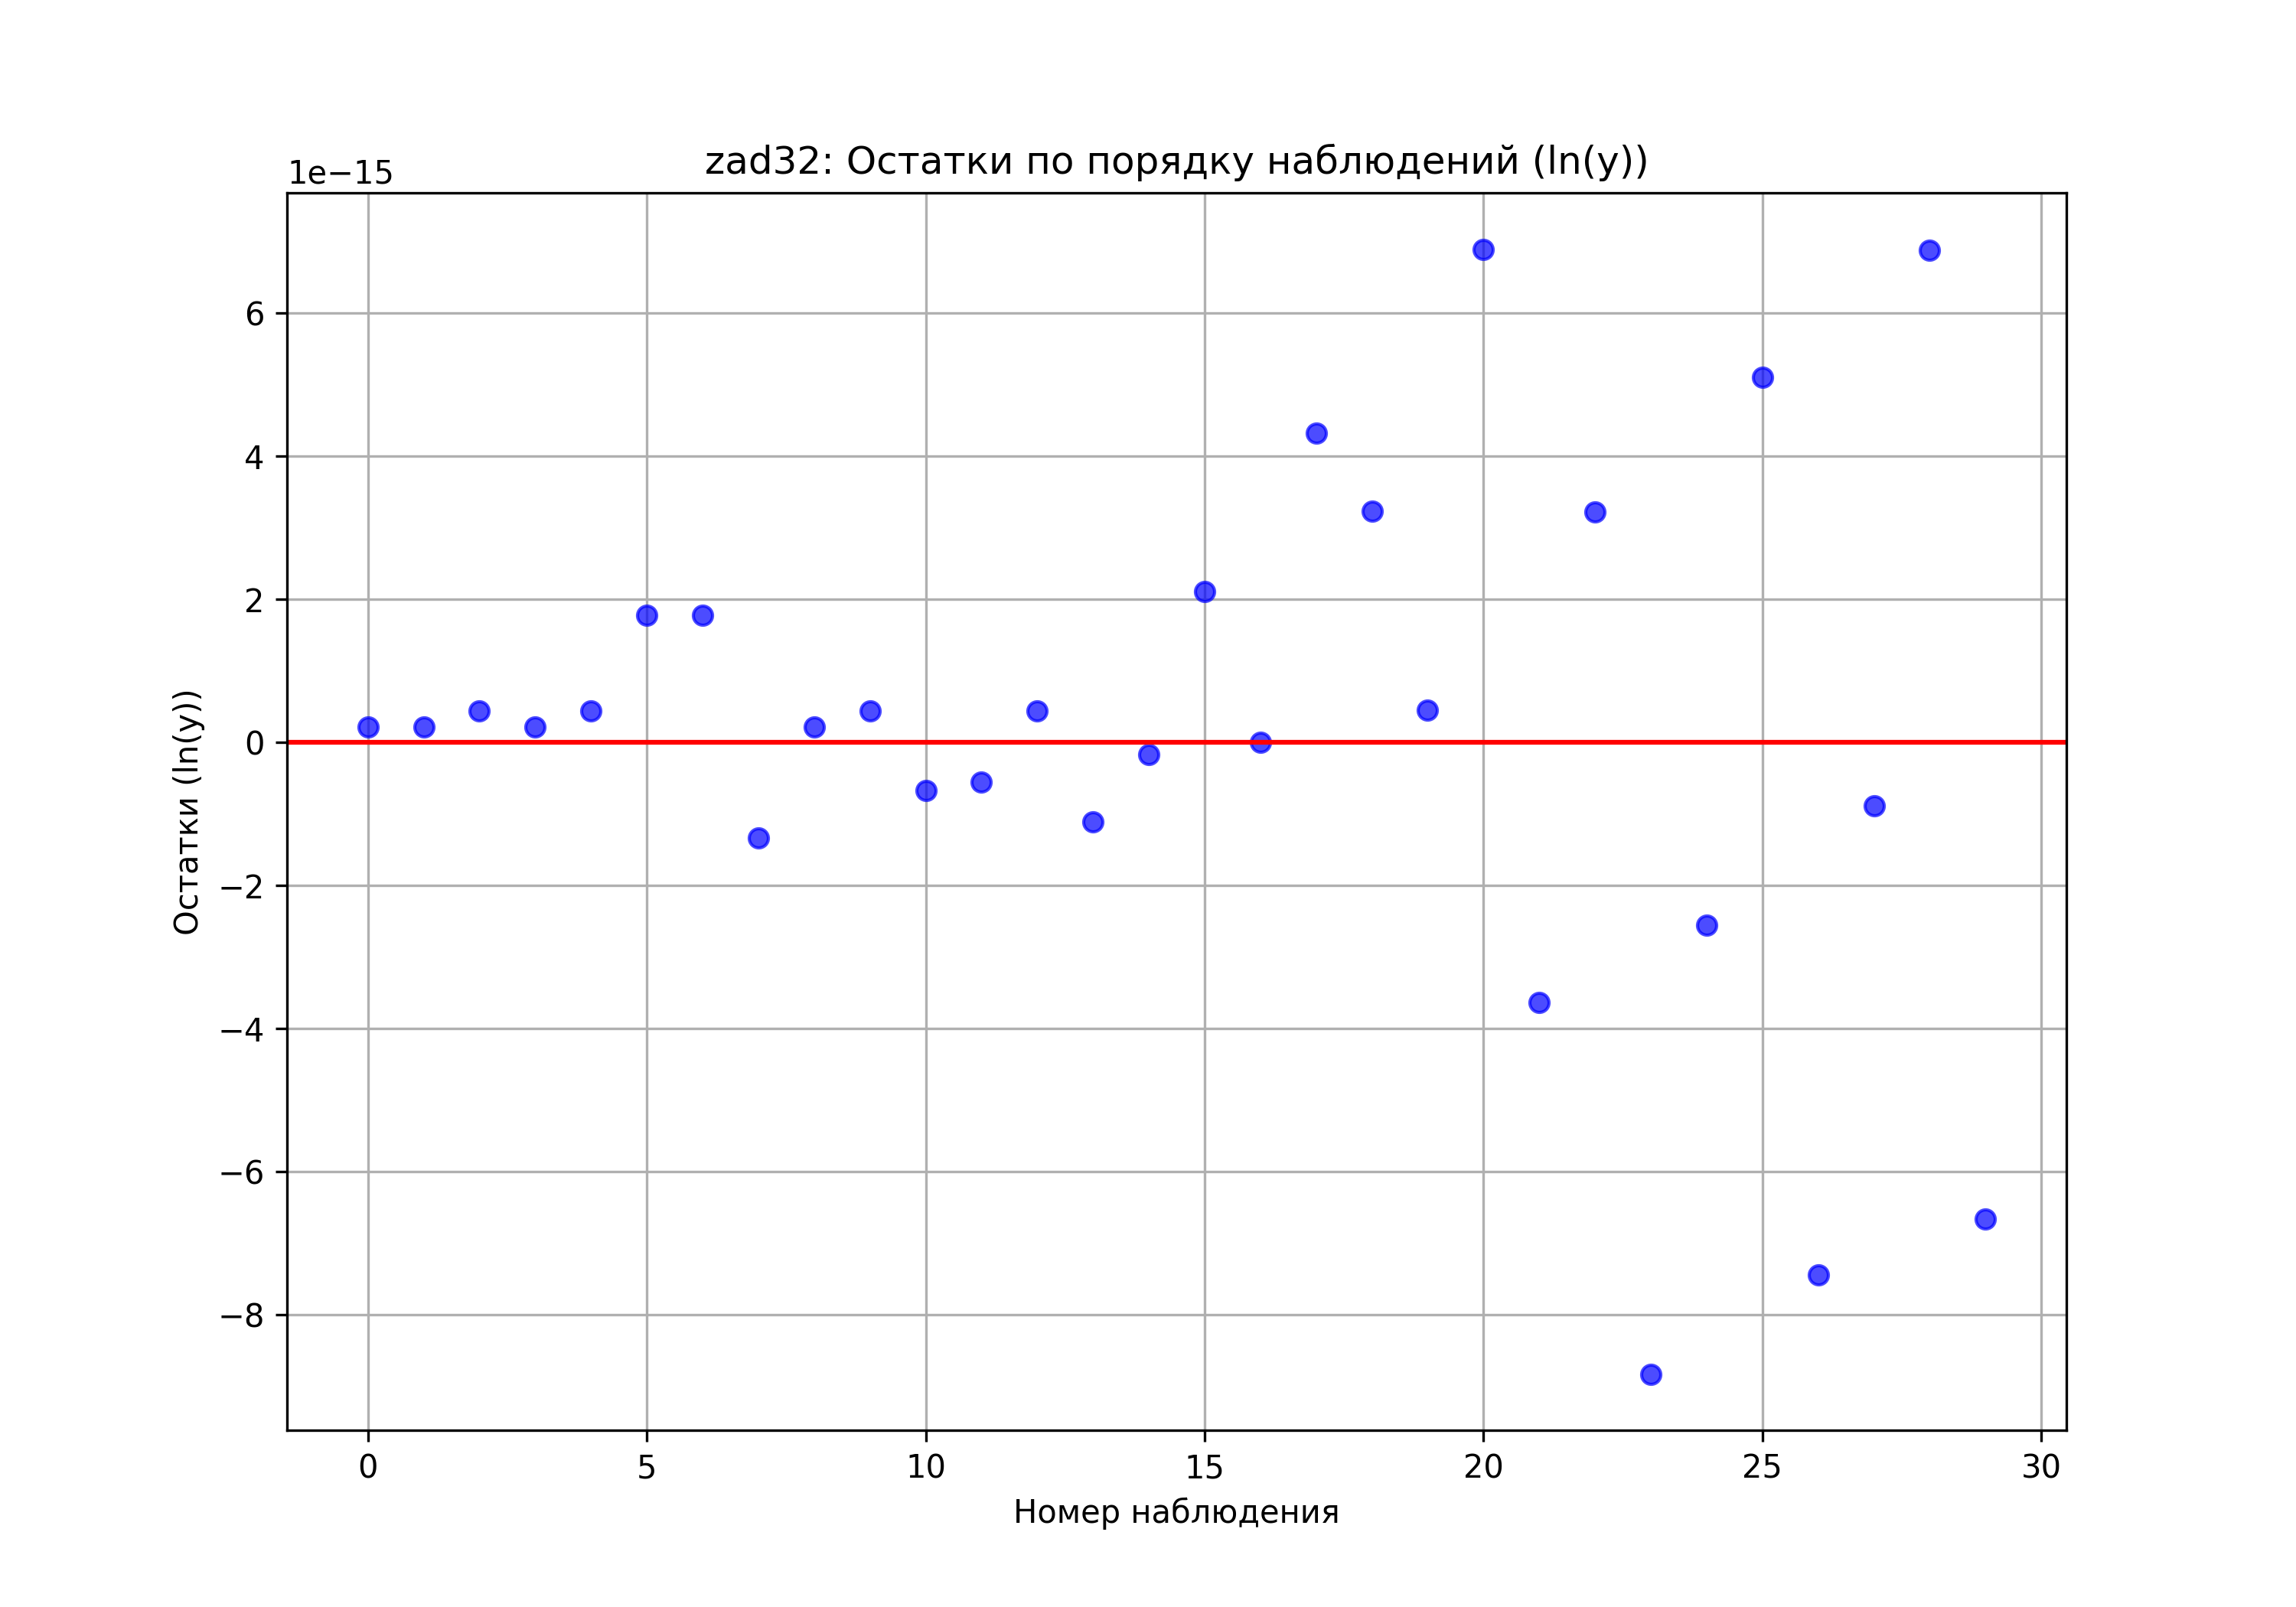
\includegraphics[width=0.8\textwidth]{fig/zad32_residuals_order.png}
\caption{Анализ автокорреляции остатков}
\label{fig:zad32_residuals_order}
\end{figure}

\subsubsection{Проверка предпосылок теоремы Гаусса–Маркова}

\begin{enumerate}
    \item \textbf{Линейность по параметрам:} модель $z = c + d x$ линейна по вектору параметров $\boldsymbol{\beta} = (c, d)^\top$, условие выполнено.

    \item \textbf{Случайный отбор наблюдений:} предполагается, что наблюдения независимы. При нарушении возможна автокорреляция, которая делает стандартные ошибки несостоятельными.

    \item \textbf{Нулевое математическое ожидание ошибок:} проверено с использованием $t$-статистики:
    \[
    H_0: \mathbb{E}[\varepsilon_i] = 0.
    \]
    Получено $t = 0.2350$, $p = 0.8158 > 0.05$, гипотеза $H_0$ не отвергается.

    \item \textbf{Гомоскедастичность:} Тест Бреуша–Пагана:
    \[
    H_0: \operatorname{Var}(\varepsilon_i) = \sigma^2, \quad H_1: \operatorname{Var}(\varepsilon_i) \text{ зависит от } x_i.
    \]
    Результат: $\chi^2 = 12.0790$, $p = 0.0005 < 0.05$, $H_0$ отвергается. Имеется гетероскедастичность, что нарушает эффективность МНК-оценки.

    \item \textbf{Отсутствие автокорреляции:} Проверено с помощью:
    \begin{itemize}
        \item Теста Дарбина–Уотсона: $DW = 2.5197$.
        \item Теста Льюнга–Бокса: $Q = 3.4834$, $p = 0.0620$.
    \end{itemize}
    При уровне значимости $\alpha = 0.05$ гипотеза об отсутствии автокорреляции формально не отвергается, однако $p$-значение близко к пороговому.

    \item \textbf{Мультиколлинеарность:} Вычислены факторы инфляции дисперсии:
    \[
    \text{VIF}_{\text{const}} = 3.8065, \quad \text{VIF}_{x} = 1.0000.
    \]
    Поскольку $\max(\text{VIF}) < 10$, мультиколлинеарности не наблюдается.
\end{enumerate}

\begin{remark}
Ввиду выявленной гетероскедастичности, оценки параметров $\hat{c}$, $\hat{d}$ сохраняют несмещённость, но теряют эффективность.
\end{remark}

\begin{answer}
Проведённое преобразование позволило свести задачу нелинейной регрессии к линейной по параметрам. В условиях нарушенной гомоскедастичности, оценки МНК сохраняют свойства несмещённости, однако теряют эффективность. Остальные предпосылки теоремы Гаусса–Маркова не отвергнуты статистическими тестами. Следовательно, полученные оценки параметров можно интерпретировать как состоятельные при соответствующей корректировке стандартных ошибок.
\end{answer}

